% Generated by experiments/run_report_artifacts.py; do not edit by hand.
% Result command: python -u experiments/run_report_artifacts.py results --only long_vertical_transition
% Result file: results/long_vertical_transition_summary.csv
\begin{figure}[h]
\centering
\small
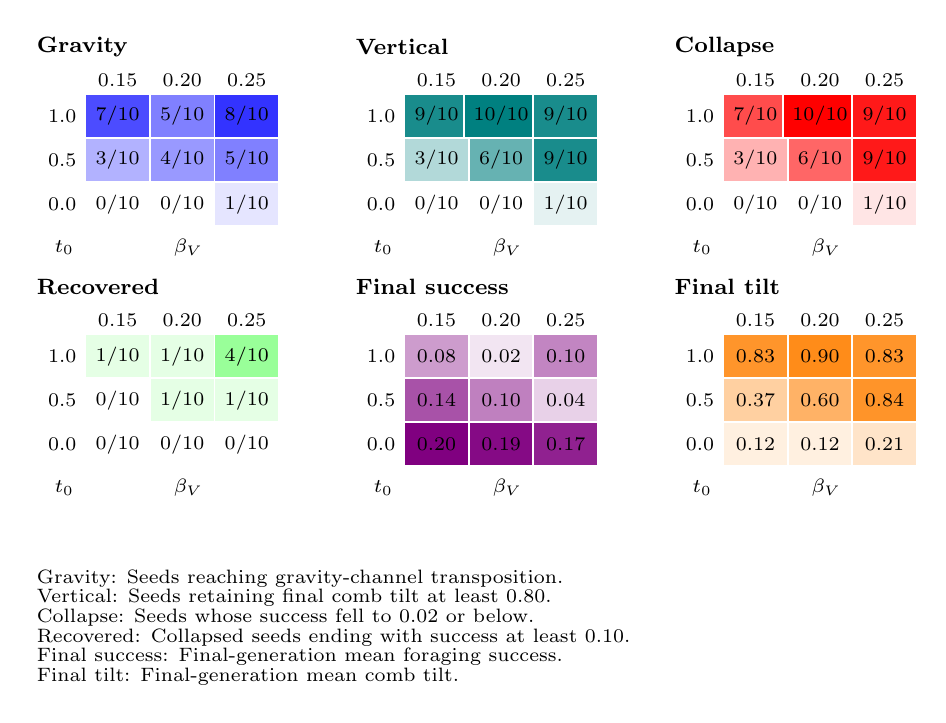
\begin{tikzpicture}[
  cell/.style={minimum width=0.82cm, minimum height=0.56cm, anchor=center, draw=white, line width=0.7pt, font=\scriptsize},
  paneltitle/.style={font=\footnotesize\bfseries, anchor=west},
  axislabel/.style={font=\scriptsize},
  legend/.style={font=\scriptsize, anchor=west}
]
\node[paneltitle] at (0.00,0.00) {Gravity};
\node[axislabel, anchor=east] at (0.72,-2.55) {$t_0$};
\node[axislabel] at (2.05,-2.55) {$\beta_V$};
\node[axislabel] at (1.15,-0.43) {0.15};
\node[axislabel] at (1.97,-0.43) {0.20};
\node[axislabel] at (2.79,-0.43) {0.25};
\node[axislabel, anchor=east] at (0.75,-0.88) {1.0};
\node[cell, fill=blue!70!white] at (1.15,-0.88) {7/10};
\node[cell, fill=blue!50!white] at (1.97,-0.88) {5/10};
\node[cell, fill=blue!80!white] at (2.79,-0.88) {8/10};
\node[axislabel, anchor=east] at (0.75,-1.44) {0.5};
\node[cell, fill=blue!30!white] at (1.15,-1.44) {3/10};
\node[cell, fill=blue!40!white] at (1.97,-1.44) {4/10};
\node[cell, fill=blue!50!white] at (2.79,-1.44) {5/10};
\node[axislabel, anchor=east] at (0.75,-2.00) {0.0};
\node[cell, fill=blue!0!white] at (1.15,-2.00) {0/10};
\node[cell, fill=blue!0!white] at (1.97,-2.00) {0/10};
\node[cell, fill=blue!10!white] at (2.79,-2.00) {1/10};
\node[paneltitle] at (4.05,0.00) {Vertical};
\node[axislabel, anchor=east] at (4.77,-2.55) {$t_0$};
\node[axislabel] at (6.10,-2.55) {$\beta_V$};
\node[axislabel] at (5.20,-0.43) {0.15};
\node[axislabel] at (6.02,-0.43) {0.20};
\node[axislabel] at (6.84,-0.43) {0.25};
\node[axislabel, anchor=east] at (4.80,-0.88) {1.0};
\node[cell, fill=teal!90!white] at (5.20,-0.88) {9/10};
\node[cell, fill=teal!100!white] at (6.02,-0.88) {10/10};
\node[cell, fill=teal!90!white] at (6.84,-0.88) {9/10};
\node[axislabel, anchor=east] at (4.80,-1.44) {0.5};
\node[cell, fill=teal!30!white] at (5.20,-1.44) {3/10};
\node[cell, fill=teal!60!white] at (6.02,-1.44) {6/10};
\node[cell, fill=teal!90!white] at (6.84,-1.44) {9/10};
\node[axislabel, anchor=east] at (4.80,-2.00) {0.0};
\node[cell, fill=teal!0!white] at (5.20,-2.00) {0/10};
\node[cell, fill=teal!0!white] at (6.02,-2.00) {0/10};
\node[cell, fill=teal!10!white] at (6.84,-2.00) {1/10};
\node[paneltitle] at (8.10,0.00) {Collapse};
\node[axislabel, anchor=east] at (8.82,-2.55) {$t_0$};
\node[axislabel] at (10.15,-2.55) {$\beta_V$};
\node[axislabel] at (9.25,-0.43) {0.15};
\node[axislabel] at (10.07,-0.43) {0.20};
\node[axislabel] at (10.89,-0.43) {0.25};
\node[axislabel, anchor=east] at (8.85,-0.88) {1.0};
\node[cell, fill=red!70!white] at (9.25,-0.88) {7/10};
\node[cell, fill=red!100!white] at (10.07,-0.88) {10/10};
\node[cell, fill=red!90!white] at (10.89,-0.88) {9/10};
\node[axislabel, anchor=east] at (8.85,-1.44) {0.5};
\node[cell, fill=red!30!white] at (9.25,-1.44) {3/10};
\node[cell, fill=red!60!white] at (10.07,-1.44) {6/10};
\node[cell, fill=red!90!white] at (10.89,-1.44) {9/10};
\node[axislabel, anchor=east] at (8.85,-2.00) {0.0};
\node[cell, fill=red!0!white] at (9.25,-2.00) {0/10};
\node[cell, fill=red!0!white] at (10.07,-2.00) {0/10};
\node[cell, fill=red!10!white] at (10.89,-2.00) {1/10};
\node[paneltitle] at (0.00,-3.05) {Recovered};
\node[axislabel, anchor=east] at (0.72,-5.60) {$t_0$};
\node[axislabel] at (2.05,-5.60) {$\beta_V$};
\node[axislabel] at (1.15,-3.48) {0.15};
\node[axislabel] at (1.97,-3.48) {0.20};
\node[axislabel] at (2.79,-3.48) {0.25};
\node[axislabel, anchor=east] at (0.75,-3.93) {1.0};
\node[cell, fill=green!10!white] at (1.15,-3.93) {1/10};
\node[cell, fill=green!10!white] at (1.97,-3.93) {1/10};
\node[cell, fill=green!40!white] at (2.79,-3.93) {4/10};
\node[axislabel, anchor=east] at (0.75,-4.49) {0.5};
\node[cell, fill=green!0!white] at (1.15,-4.49) {0/10};
\node[cell, fill=green!10!white] at (1.97,-4.49) {1/10};
\node[cell, fill=green!10!white] at (2.79,-4.49) {1/10};
\node[axislabel, anchor=east] at (0.75,-5.05) {0.0};
\node[cell, fill=green!0!white] at (1.15,-5.05) {0/10};
\node[cell, fill=green!0!white] at (1.97,-5.05) {0/10};
\node[cell, fill=green!0!white] at (2.79,-5.05) {0/10};
\node[paneltitle] at (4.05,-3.05) {Final success};
\node[axislabel, anchor=east] at (4.77,-5.60) {$t_0$};
\node[axislabel] at (6.10,-5.60) {$\beta_V$};
\node[axislabel] at (5.20,-3.48) {0.15};
\node[axislabel] at (6.02,-3.48) {0.20};
\node[axislabel] at (6.84,-3.48) {0.25};
\node[axislabel, anchor=east] at (4.80,-3.93) {1.0};
\node[cell, fill=violet!39!white] at (5.20,-3.93) {0.08};
\node[cell, fill=violet!10!white] at (6.02,-3.93) {0.02};
\node[cell, fill=violet!48!white] at (6.84,-3.93) {0.10};
\node[axislabel, anchor=east] at (4.80,-4.49) {0.5};
\node[cell, fill=violet!68!white] at (5.20,-4.49) {0.14};
\node[cell, fill=violet!50!white] at (6.02,-4.49) {0.10};
\node[cell, fill=violet!18!white] at (6.84,-4.49) {0.04};
\node[axislabel, anchor=east] at (4.80,-5.05) {0.0};
\node[cell, fill=violet!100!white] at (5.20,-5.05) {0.20};
\node[cell, fill=violet!96!white] at (6.02,-5.05) {0.19};
\node[cell, fill=violet!87!white] at (6.84,-5.05) {0.17};
\node[paneltitle] at (8.10,-3.05) {Final tilt};
\node[axislabel, anchor=east] at (8.82,-5.60) {$t_0$};
\node[axislabel] at (10.15,-5.60) {$\beta_V$};
\node[axislabel] at (9.25,-3.48) {0.15};
\node[axislabel] at (10.07,-3.48) {0.20};
\node[axislabel] at (10.89,-3.48) {0.25};
\node[axislabel, anchor=east] at (8.85,-3.93) {1.0};
\node[cell, fill=orange!83!white] at (9.25,-3.93) {0.83};
\node[cell, fill=orange!90!white] at (10.07,-3.93) {0.90};
\node[cell, fill=orange!83!white] at (10.89,-3.93) {0.83};
\node[axislabel, anchor=east] at (8.85,-4.49) {0.5};
\node[cell, fill=orange!37!white] at (9.25,-4.49) {0.37};
\node[cell, fill=orange!60!white] at (10.07,-4.49) {0.60};
\node[cell, fill=orange!84!white] at (10.89,-4.49) {0.84};
\node[axislabel, anchor=east] at (8.85,-5.05) {0.0};
\node[cell, fill=orange!12!white] at (9.25,-5.05) {0.12};
\node[cell, fill=orange!12!white] at (10.07,-5.05) {0.12};
\node[cell, fill=orange!21!white] at (10.89,-5.05) {0.21};
\node[legend] at (0.0,-6.75) {Gravity: Seeds reaching gravity-channel transposition.};
\node[legend] at (0.0,-7.00) {Vertical: Seeds retaining final comb tilt at least 0.80.};
\node[legend] at (0.0,-7.25) {Collapse: Seeds whose success fell to 0.02 or below.};
\node[legend] at (0.0,-7.50) {Recovered: Collapsed seeds ending with success at least 0.10.};
\node[legend] at (0.0,-7.75) {Final success: Final-generation mean foraging success.};
\node[legend] at (0.0,-8.00) {Final tilt: Final-generation mean comb tilt.};
\end{tikzpicture}
\caption{Long axial-orientation transition experiment. Rows are initial comb tilt, columns are vertical-comb benefit. Count panels report seeds out of ten; continuous panels report final-generation means. The generated fragment records the source CSV.}
\label{fig:long-transition-heatmap}
\end{figure}
